\section{Implementation}
\label{sec:implementation}
In this section, we discuss the implementation of the proposed approach. 
Figure~\ref{fig:transformationWorkflow} shows the transformations workflow. Each transformation is identified by a number (1-7 in Figure~\ref{fig:transformationWorkflow}) for easier reference. 
In addition to the transformations, supporting files needed for the creation of the Papyrus plugin are also generated while icons and shapes are placed next to the annotated metamodel (\#8 in Figure~\ref{fig:transformationWorkflow}). 
As the transformations consists of about 1000 lines of code we will describe them omitting low level technical details\footnote{Full implementations and instructions are available at \url{http://www.zolotas.net/AMIGO/}}. 

\begin{figure*}[t]
	\centering
	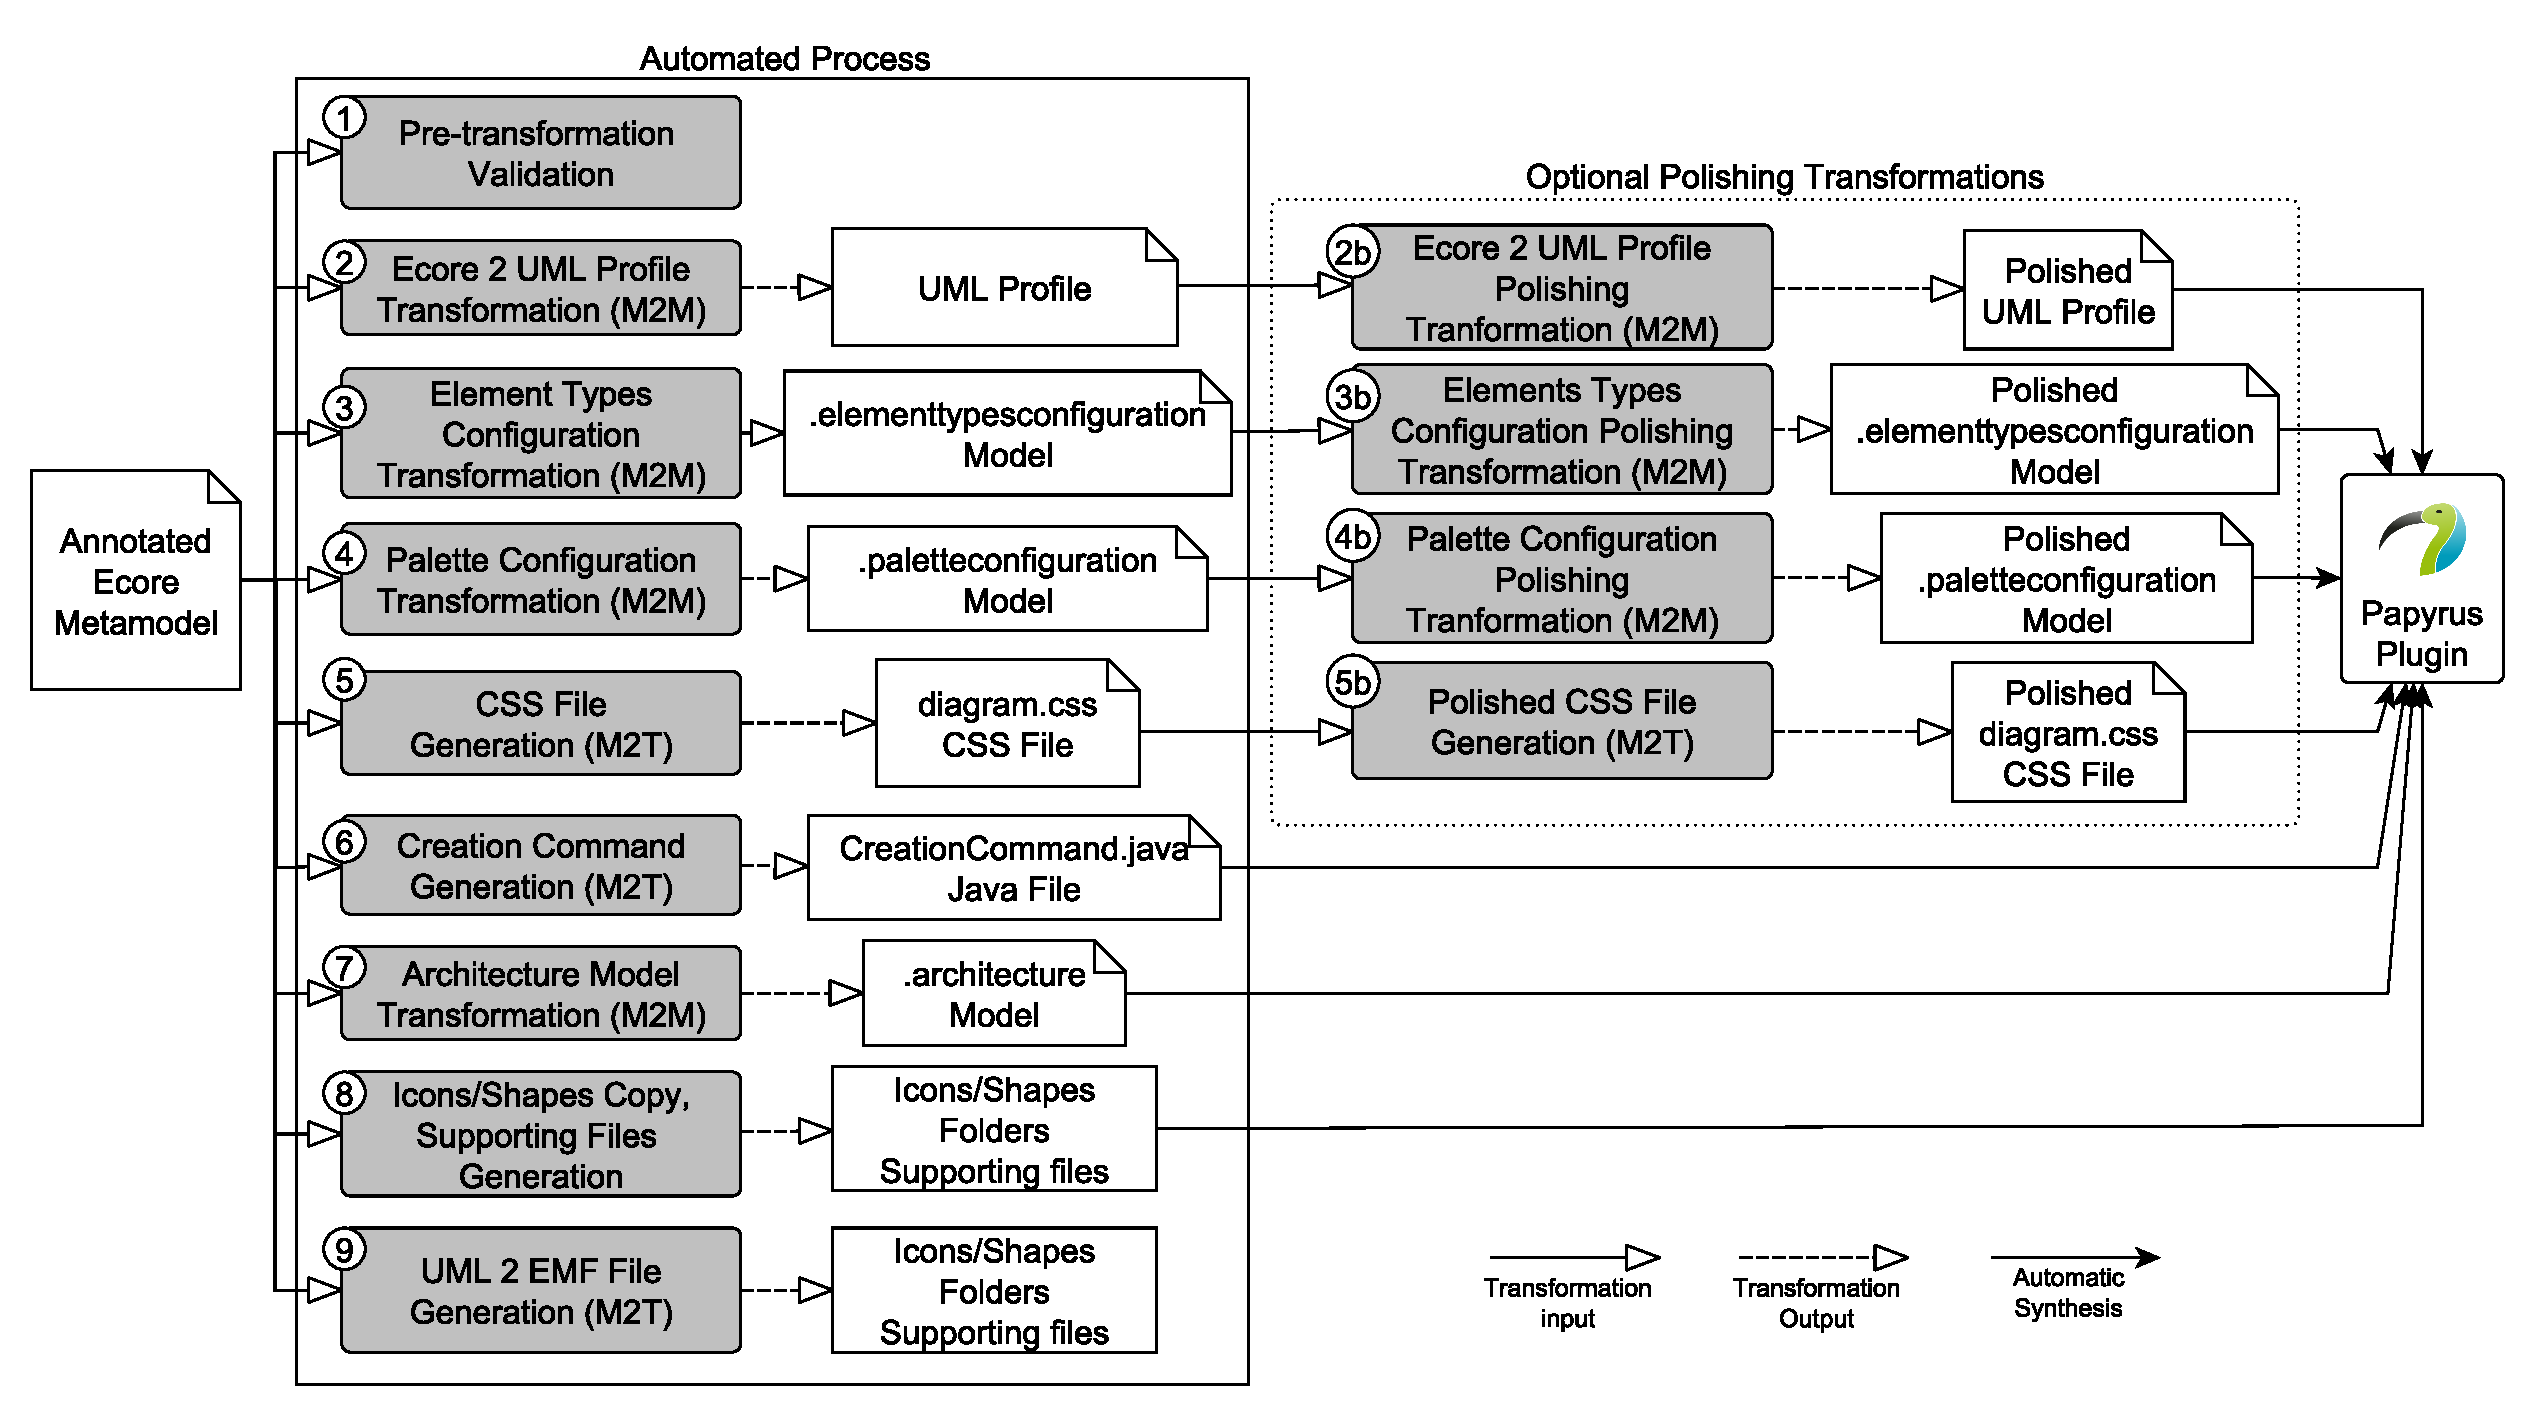
\includegraphics[width=1	\textwidth]{diagrams/transformationWorkflow.pdf}
	\caption[]{An overview of the transformation workflow}
	\label{fig:transformationWorkflow}
	\vspace*{-3mm}
\end{figure*}

\subsection{EMF to UML Profile Generation (\#1)}
\label{sec:profileGeneration}
This transformation consists of two rules, one that creates one stereotype for each EClass element of the metamodel and a second that creates a stereotype for EReferences annotated as @Edge. 
The source model of this transformation is the annotated Ecore metamodel (e.g,  Listing~\ref{lst:annotatedSdplEmfatic}) and the target model is a UML profile model.
%\footnote{UML profiles in Papyrus are actually EMF models that are instances of the UML's EMF metamodel}. 

\begin{itemize}
	\item[--] \textbf{rule eclass2stereotype:} This transformation rule transforms each EClass element in the Ecore metamodel to an element of type \textit{Stereotype} in the target UML model. All the attributes of each EClass are also copied across to the created stereotype.  
	\item[--] \textbf{rule reference2stereotype:} This rule creates a new \textit{Stereotype} with the same name in the UML profile model for each of the \textit{EReferences} that are annotated as @Edge in the Ecore metamodel. No attributes are added to the stereotype as EReferences do not support attributes in Ecore. 
\end{itemize}

When all stereotypes are created, a number of post-transformation operations are executed to 1) create the generalisation relationships between the 
stereotypes, 2) add the references/containment relationships between the stereotypes, 3) create the extension with the UML base meta-element and 4) 
generate and add the needed OCL constraints for each edge: 

\begin{enumerate}[label=\arabic*)]
	\item For each of the superclasses of an EClass in the metamodel we create a \textit{Generalisation} UML element. 
	The generalisation element is added to the stereotype created for this specific EClass and refers via the \textit{generalization} reference to the stereotype that was created for the superclass.
	\item For each reference (ref or val) in the metamodel a new \textit{Property} UML element is created and added to the stereotype that 
	represents the EClass. 
	A new \textit{Association} UML element should also be created and added to the stereotype. The name and the multiplicities are also set.
	\item By default the stereotypes extend the \textit{Class} base element unless a different value is passed in the \textit{base} property of the @Node/@Edge annotation. 
	In this post-transformation operation the necessary \textit{Import Metaclass} element and \textit{Extension} reference are created and attached to the stereotype.
	\item In the last operation,  the OCL constraints are created for each stereotype that will be represented as an edge on the diagram. 
	Two \textit{Constraint} and two \textit{OpaqueExpression} elements are created for each edge stereotype that check the two necessary constraints. 
	The OCL constraints are explained in details in the section that follows.
\end{enumerate}

\subsection{Constraints}
\label{sec:constraints}

To illustrate the OCL constraints, we provide a partial view of the SDPL UML profile in Figure \ref{fig:sample_profile}\footnote{The attributes of the stereotypes are omitted for simplicity.}.

\begin{figure}[ht!]
	\centering
	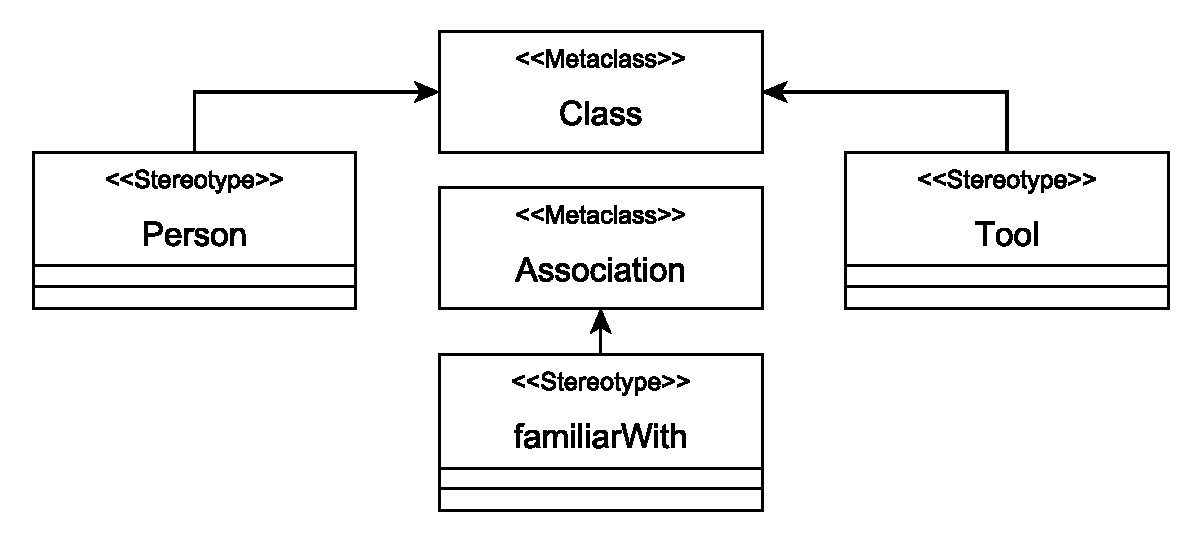
\includegraphics[width=0.5\textwidth]{diagrams/example_profile}
	\caption[]{Example UML profile for SDPL showing Person, Tool and the familiarWith association}
	\label{fig:sample_profile}
\end{figure}

In Figure \ref{fig:sample_profile}, there are three \emph{Stereotype}s - 
\emph{Person} and \emph{Tool}, both extend the meta-element \emph{UML::Class}, 
and they correspond to classes \emph{Person} and \emph{Tool} in the Emfatic 
code in Listing \ref{lst:annotatedSdplEmfatic}. \emph{Stereotype} 
\emph{familiarWith}, which extends meta-element \emph{UML::Association}, 
corresponds to the reference \emph{familiarWith} in the \emph{Person} class in 
Listing \ref{lst:annotatedSdplEmfatic}.

%
%\begin{figure}[ht!]
%	\centering
%	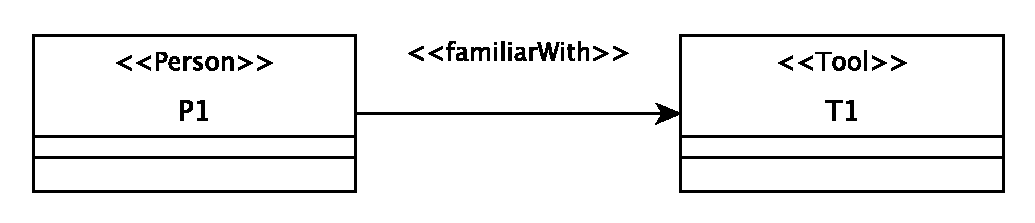
\includegraphics[width=0.5\textwidth]{diagrams/example_class_diagram}
%	\caption[]{Example Class diagram using SDPL UML Profile}
%	\label{fig:sample_class}
%\end{figure}

In Figure~\ref{fig:sdplEditor}, the \textit{familiarWith} association is used 
to connect \textit{Person} \emph{Alice} with \textit{Tool} \emph{StarUML}. However, 
the \emph{familiarWith} stereotype can be applied to any \emph{Association}, 
and not strictly to \emph{Associations} which connect \emph{Person} and 
\emph{Tool} stereotyped elements. Therefore, constraints are needed to check 
(at least) two aspects:

\begin{itemize}
	\item \textbf{End Types}: the elements that a \emph{familiarWith} association connects to that have \emph{Person} and \emph{Tool} stereotypes applied to them;
	\item \textbf{Navigability}: the \emph{familiarWith} association starts from an element stereotyped as \emph{Person} and points to an element stereotyped as \emph{Tool}.
\end{itemize}

\subsubsection{End Types}
Listing \ref{lst:endTypes} shows the OCL code for the \emph{End Types} constraint. Line 1 accesses the types that \emph{familiarWith} connects. Lines 3 and 4 check if the types that \emph{familiarWith} connects are of type that either has stereotype \emph{Person} or \emph{Tool}. In this way, if a \emph{familiarWith} association connects two types that are not \emph{Person} or \emph{Tool}, the constraint fails.

%In UML profiling, meta-element extensions are associations (instead of generalisations)

\lstinputlisting[caption={The End Types constraint in OCL},label={lst:endTypes}, captionpos=b, language=OCL, tabsize=2, numbers=left, numbersep=5pt, numberstyle=\tiny, breaklines=true, escapeinside={(*}{*)}]{endtypes.txt}

\subsubsection{Navigability}
Listing \ref{lst:navigability} shows the OCL code for the \emph{Navigability} constraint. In this case, we are interested in checking the \emph{isNavigable} property of each end. Thus, in lines 2 and 3, we obtain the member ends that \emph{familiarWith} connects with. If these ends are obtained successfully (line 4), we check that the \emph{personEnd} (connecting element stereotyped as \emph{Person}) is not navigable (line 5) and the \emph{toolEnd} (connecting element stereotyped as \emph{Tool}) is navigable (line 6). Therefore, we are checking that a \emph{familiarWith} association can only go from \emph{Person} to \emph{Tool} and not the other way around. We need to highlight, that currently, opposite references are not supported; plans for future work are outlined in Section~\ref{sec:future}.

\begin{figure}[h]
	\lstinputlisting[caption={The Navigability constraint in 
		OCL},label={lst:navigability}, captionpos=b, language=OCL, tabsize=2, 
	numbers=left, numbersep=5pt, numberstyle=\tiny, breaklines=true, 
	escapeinside={(*}{*)}]{navigability.txt}
	
	\vspace*{-5mm}
\end{figure}

With these two constraints implemented, we are able to automatically generate 
OCL constraints for stereotypes that extend \emph{UML::Association}. We use the 
\emph{End Types} and \emph{Navigability} constraints as templates with dynamic 
sections (where the specific stereotype names are inserted dynamically, e.g., 
\emph{Person} and \emph{Tool}). So far we have only explored stereotypes that 
extend \emph{UML::Association}. The constraint templates for stereotypes that 
extend other UML relationships need to be developed separately as the means to 
access source/target elements of the relationship are different.




\subsection{Palette Generation (\#2)}
\label{sec:paletteGeneration}
This transformation is responsible for creating a model (of extension.paletteconfiguration) that configures the contents of the custom palette for 
the diagram in Papyrus. 
The model conforms to the \textit{PaletteConfiguration} metamodel that ships with Papyrus. 
The transformation creates a new \textit{PaletteConfiguration} element and adds two new \textit{DrawerConfiguration} elements that represent the two different tool compartments in our palette (i.e., one for the tools that create nodes and one for those creating edges). 
For each element in the Ecore source annotated as @Node/@Edge a new \textit{ToolConfiguration} element is created and added to the nodes/edges drawer respectively. 
An \textit{IconDescriptor} element is also created and added to the ToolConfiguration pointing to the path of the icon for that tool (this is the path passed as argument to the \textit{icon} property of the @Node/@Edge annotation).

\subsection{Diagram Configuration (\#3, \#4 \& \#5)}
\label{sec:diagramConfiguration}
Firstly, in order for Papyrus to offer the choice of creating new custom diagrams for the generated profile via its menus, a \textit{Viewpoint Configuration} needs to be created. 
This creates a new entry in the ``New Diagram'' menu of Papyrus, hides the default palette and attaches the custom one created for the profile (see transformation \#2). 
It is also responsible for binding the generated CSS stylesheet file (see transformation \#6) to the diagram. 
The transformation (i.e., \#3) creates a new model that conforms to the \textit{Configuration} metamodel that ships with Papyrus. 
A new \textit{Viewpoint Configuration} element is created that sets the visibility of the default palette (via the \textit{permit} attribute) to false. 
It also populates the value of the \textit{Custom Palette} feature to point to the \emph{.paletteconfiguration} file created by transformation \#2. Finally, it sets the value of the \textit{Custom Style} attribute to point to the CSS file generated by transformation \#6.

The second artefact that needs to be created is the types configuration model (i.e., .typesconfiguration file) that conforms to the \textit{Element Types 
Configuration} metamodel provided by Papyrus. 
This is achieved through transformation \#4. This model is responsible for binding the types of the drawn elements to stereotypes. 
For each stereotype a new element of type \textit{Specialization Type Configuration} is created and a unique \textit{id} is created in the format ``ProfileName.StereotypeName'' (e.g., ``SDPL.Step''). 
The value of the \textit{Hint} attribute is set to the qualified name of the meta-element that this type specialises (e.g., ``UML::Class''). 
A new element of type \textit{Stereotype Application Matcher Configuration} is also created that holds the qualified name of the stereotype that should be applied to the drawn element. 
Binding is performed by creating a new \textit{Apply Stereotype Advice Configuration} element for each stereotype that points to the equivalent stereotype application matcher configuration element created before. 
Having this file, when an element of a specific type is drawn the appropriate stereotype is applied automatically. 

The last model (i.e., the .elementtypesconfiguration file) that needs to be created for the custom diagram is the elements types configuration that 
conforms to the \textit{Element Types Configuration} metamodel available in Papyrus. 
This is done by transformation \#5. As all the stereotypes created extend a UML meta-element, this model is responsible for specializing the meta-element \textit{shapes} to the custom ones created by the profile. 
Thus, for each stereotype, a new \textit{Specialization Type Configuration} element is created. 
This element points to the two elements that it specializes: the specialization type configuration created in transformation \#4 via its id (e.g., ``Process.Step'') and the shape of the UML meta-element that this element specializes via its uri (e.g., ``org.eclipse.papyrus.umldi.Class\_Shape'').

\subsection{Stylesheet Generation (\#6)}
\label{sec:cssGeneration}
As stated above, in Papyrus, the look and feel of diagram elements can be customised using CSS. 
In this transformation we generate the CSS style rules that define the appearance of nodes and edges in diagrams. 
Each node on a diagram has a set of compartments where the attributes, the shape, etc. appear. 
Initially, for all the nodes that will appear on the diagram, we create a CSS rule to hide all their compartments and another rule to enable the compartment that holds the shape. 
The latter rule also hides the default shape inherited from the meta-element tat the stereotype extends. 
Then, for each stereotype that appears as a node, a CSS rule is generated to place the SVG figure in the shape compartment. 
For elements of type \textit{Stereotype}, the connection of the SVG figure to the stereotypes is achieved by assigning the path of the SVG file to the 
\textit{svgFile} property available in CSS. 
Finally, we generate the CSS rules for each edge, e.g., if a \emph{lineStyle} parameter is set, then the \textit{style} property for that Edge stereotype is set to the value of the lineStyle parameter (e.g., ``solid'', ``dashed'', etc.).

\subsection{UML to EMF Transformation Generation (\#7)}
\label{sec:uml2emf}
This M2T transformation generates the ETL file that can be used to transform the UML models created in Papyrus and conform to the UML Profile generated by 
our approach, back to EMF models that conform to the source Ecore metamodel given as input to the approach. 
One rule is generated for each of the stereotypes that transforms them back to the appropriate type of the Ecore metamodel. 
Each stereotype has the same attributes and references as the original EClass thus, this EGL script also generates the statements in each rule that populate the attributes and the references of the newly created instance of each EClass with the equivalent values of the UML model. 
An example of an auto-generated rule is shown in Listing~\ref{lst:etlGeneratedRule}. 
This rule transforms elements stereotyped as ``Person'' in the UML model to elements of type ``Person'' in an EMF model which conforms to the Ecore metamodel presented in Listing~\ref{lst:annotatedSdplEmfatic}.

\lstinputlisting[caption={Example of an auto-generated ETL rule that transforms \\elements stereotyped as ``Person'' in the UML model to elements of \\type ``Person'' in an EMF model.},label={lst:etlGeneratedRule},captionpos=b, language=ETL, tabsize=2, numbers=left, numbersep=5pt, numberstyle=\tiny, breaklines=true]{etlExample.etl}

%Epsilon Transformation Language (ETL) \cite{} is a hybrid model-to-model transformation languages which provides both a declarative rule-based execution scheme and imperative features for handling complex transformation scenarios. In Listing~\ref{lst:etlGeneratedRule}, rule \emph{PersonUML2PersonEMF} is responsible to transform a \emph{Person} in the UML model to a \emph{Person} in the EMF model. 

ETL provides the $::=$ operator for rule resolution. 
The ETL engine keeps transformation traces which links source elements to target elements of the transformation. 
When $::=$ is used, the ETL execution engine inspects the established transformation traces and invokes the applicable rules (if necessary) to calculate the counterparts of the source elements contained in the collection. 

%If \emph{equivalents()} is applied to a single element, it returns a collection which contains the counterpart(s) of the element in the target model. If \emph{equivalents()} is applied to a collection of elements, it returns a collection of collection (each collection in the result contains the counterparts of the element in the target model). 

In our example (line 6 in Listing \ref{lst:etlGeneratedRule}), the expression ``s.familiarWith'' returns a collection of \emph{UMLProcess!Tool}s (denoted by $ct$). By using ``::='', the ETL engine will look for the rules that transform \emph{UMLProcess!Tool} to \emph{EMFProcess!Tool} and invoke the rules if 
necessary (if the source elements have not been transformed, as shown in the transformation trace) and put the transformed elements into sub-collections 
(denoted by $sc$). 
After the ETL engine goes through all the elements in $ct$, the sub-collections $sc$s are returned (flattened to a single collection if more than one) and are added to ``t.familiarWith''.

\subsection{Icons, Shapes and Supporting Files (\#8)}
\label{sec:supportingFiles}
The approach supports the generation of the UML profile and the infrastructure for the Papyrus diagram in either a new plugin project or in the same plugin project where the annotated Ecore metamodel resides. 
In both scenarios, the ``MANIFEST.MF'', the ``build.properties'' and the ``plugin.xml'' files are created (or overridden respectively). 
The first includes the list of all the required bundles while the second points the project to the locations of the ``MANIFEST.MF'' and ``plugin.xml'' files. 
The third (i.e., ``plugin.xml'') includes all the necessary extensions for Papyrus to be able to register the UML profile and create the diagrams (e.g., extensions that point to the diagrams.configuration, .elementtypesconfiguration, .typesconfiguration, etc. files). 

For the scenario where the Papyrus plugin is created as a new project, the shapes (SVG files) and the icons (PNG files) are copied to the newly created 
plugin project. 
For the scenario where the UML profile and editor is generated in the same project in which the Ecore source file resides, the shapes and icons files do not need to be copied as they already exist.

Finally, two files that only consist of the XML and the XMI header (namely ``model.profile.di'' and ``model.profile.notation'') are generated. These files are necessary for Papyrus to construct the UML profile model.

\subsection{Polishing Transformations (\#1b - \#6b)}
\label{sec:transformationPatches}
For each of the transformations \#1 - \#6, users are able to define polishing transformations that will complement those included in our implementation. After each built-in transformation is executed, the workflow looks to find a transformation with the same file name next to the Ecore metamodel. 
If a file with the same name exists, it is executed against the Ecore metamodel and targets the already created output model of the original transformation. 
The execution of the polishing transformation is set \textit{not} to overwrite the target model but to refine it instead.
Table~\ref{tab:polishingTransformationsNames} shows the names that each polishing transformation is expected to have.

\begin{table}[h]
	\caption{Polishing Transformations File Names}
	\centering
	\setlength{\tabcolsep}{3.5pt} 
	\begin{tabular}{|c|c|}
		\cline{1-2}
		\textbf{Transformation ID}  & \textbf{Required File Name}\\ \hline
		\textbf{\#1} & emf2umlProfile.etl\\ \hline
		\textbf{\#2} & paletteConfigurationM2M.etl\\ \hline
		\textbf{\#3} & diagramsConfigurationM2M.etl\\ \hline
		\textbf{\#4} & typesConfigurationsM2M.etl\\ \hline
		\textbf{\#5} & elementTypesConfigurationsM2M.etl\\ \hline
		\textbf{\#6} & cssFileGeneration.egl\\ \hline
		\cline{1-2}
	\end{tabular}
	\label{tab:polishingTransformationsNames}
\end{table}
